% %%%%%%%%%%%%%%%%%%%%%%%%%%%%%%%%%%%%%%%%%%%%%%%%%%%%%%%%%%%
% Hier nichts aendern
\documentclass[sigconf, nonacm, review]{acmart}
\AtBeginDocument{%
  \providecommand\BibTeX{{%
    \normalfont B\kern-0.5em{\scshape i\kern-0.25em b}\kern-0.8em\TeX}}}

\setcopyright{acmcopyright}
\copyrightyear{2018}
\acmYear{2018}
\acmDOI{XXXXXXX.XXXXXXX}
\acmJournal{JACM}
\acmVolume{37}
\acmNumber{4}
\acmArticle{111}
\acmMonth{8}
\acmPrice{15.00}
\acmISBN{978-1-4503-XXXX-X/18/06}
% Hier nichts aendern
% %%%%%%%%%%%%%%%%%%%%%%%%%%%%%%%%%%%%%%%%%%%%%%%%%%%%%%%%%%%

\begin{document}
% %%%%%%%%%%%%%%%%%%%%%%%%%%%%%%%%%%%%%%%%%%%%%%%%%%%%%%%%%%%
% Hier eigene Daten eingeben
\title{Report zum Fachprojekt Routingalgorithmen}
\author{Pouria Araghchi}
\affiliation{%
  \institution{TU Dortmund}
  \streetaddress{Otto-Hahn-Straße 14}
  \city{Dortmund}
  \country{Deutschland}}
\email{pouria.araghchi@tu-dortmund.de}

\author{Kai Lukas Ilmenau}
\affiliation{%
  \institution{TU Dortmund}
  \streetaddress{Otto-Hahn-Straße 14}
  \city{Dortmund}
  \country{Deutschland}}
\email{kai.ilmenau@tu-dortmund.de}

\author{Naveed Niazi}
\affiliation{%
  \institution{TU Dortmund}
  \streetaddress{Otto-Hahn-Straße 14}
  \city{Dortmund}
  \country{Deutschland}}
\email{naveed.niazi@tu-dortmund.de}

\renewcommand{\shortauthors}{Araghchi, Ilmenau, Niazi}
% Hier eigene Daten eingeben
% %%%%%%%%%%%%%%%%%%%%%%%%%%%%%%%%%%%%%%%%%%%%%%%%%%%%%%%%%%%

\begin{abstract}
In diesem Report werden die Ergebnisse unserer Arbeit im Rahmen des Fachprojekts "Routingalgorithmen" zusammengefasst.
Wir haben die Algorithmen auf die Maximum Link Utilization (MLU) nach \cite{foerster2021} untersucht.
\textcolor{red}{Beschreibung der Ergebnisse von Pourias Algorithmus}
Der Algorithmus, der inverse capacity mit centrality Metriken verrechnet, ist meistens schlechter als inverse capacity, 
da reines inverse capacity öfter zwei kürzste Wege finden um demands gleichmäßiger zu verteilen damit einzelne Links nicht überlastet werden.
Es wird jedoch auch gezeigt, dass Topologien gefunden werden können, bei den pures inverse capacity eine schlechtere MLU hat.
\textcolor{red}{Beschreibung der Ergebnisse von Naveeds Algorithmus}
Die Replikation andere Gruppen im ersten Projektteil nicht erfolgreich, und im zweiten schon, 
jedoch haben wir daraus die Lehre gezogen wie wir unsere Arbeit besser replizierbar machen und das frühe Kommunikation mit den anderen Gruppen wichtig ist.
\end{abstract}

\begin{CCSXML}
<ccs2012>
<concept>
<concept_id>10003033.10003068.10003073.10003076</concept_id>
<concept_desc>Networks~Traffic engineering algorithms</concept_desc>
<concept_significance>500</concept_significance>
</concept>
</ccs2012>
\end{CCSXML}

\ccsdesc[500]{Networks~Traffic engineering algorithms}

% Eventuell keywords weglassen
\keywords{weight optimization, waypoint optimization}

\received{6. August 2023}
\received[\"uberarbeitet]{\textcolor{red}{ausstehend}}
\received[akzeptiert]{15. August 2023}

\maketitle

\section{Einleitung}
In der heutigen Zeit werden mehrere Millionen Datenpakete von und zu Knotenpunkten verschickt.
Daher ist das \emph{Routing} von diesen Datenpaketen in der heutigen Zeit wichtiger denn je.
Gutes Routing kann Datenstaus verringern oder sogar verhindern, Verteilerknoten auslasten oder entlasten 
und sorgt damit fuer einen reibungslosen Datenverkehr ueberall auf der Welt.
Wie gut das Routing innerhalb einer Netzwerktopologie ist, wird durch den darunterliegenden Routingalgorithmus bestimmt.
Hierf\"ur gibt es verschiedenste Ans\"atze mit variierender Komplexit\"at und Erfolgswahrscheinlichkeit.

Deswegen haben wir uns im Rahmen des Fachprojekts "Routingalgorithmen" näher mit den verschiedenen Algorithmen beschäftigt und haben eigene Variationen dieser Algorithmen erstellt um ein tieferes Verständnis der Materie zu erlangen.
In diesem Report fassen wir die Ergebnisse unserer Arbeit zusammen.
Dies umfasst eine Beschreibung unserer algorithmischen Ideen, sowie Experimente zu diesen im Stil des paper \cite{foerster2021} und eine Einordnung der Resultate dieser Experimente.
Außerdem gehen wir auf die Arbeit einer anderen Gruppe im Fachprojekt ein, die wir versucht haben zu replizieren.

\section{Theoretische Grundlagen}
\textcolor{red}{Hier wird etwas zum Paper stehen}\cite{foerster2021}.
\section{Umsetzung}
In diesem Abschnitt werden unsere Projekte und die dazugeh\"origen Ideen vorgestellt.
Die beiden Projekte sind in Unterabschnitte und die algorithmischen Ideen und Umsetzungen des jeweiligen Gruppenmitglieds in Paragraphen unterteilt. 
\subsection{Algorithmen zu Projekt 1}
In Projekt 1 ging es darum, eine algorithmische Idee auf Basis von \cite{foerster2021} herauszuarbeiten und diese mithilfe desselben Git-Prokjekts\footnote{\url{https://github.com/fruitiestPunch/FaPro_P1}, siehe Abschnitt \ref{sec:resouces}} mit alternativen Routingalgorithmen zu vergleichen. 
\subsubsection{Sequential combination aus inverse capacity und demand first waypoints}
Der Kerngedanke hier war es, einen einen schnellen Algorithmus zu finden, 
welcher hinreichend gute Ergebnisse in Bezug auf die MLU abliefert.
Diese Eigenschaft ist insbesondere f\"ur Netzwerke sinvoll,
dessen Auslastungen sich regelm\"a\ss ig w\"ahrend des Betriebs \"andern und der ALgorithmus reaktiv sehr schnell alle Gewichte und Wegpunkte neu berechnet.\newline
Die Grundlage dieses Algorithmus war die sequentielle Kombination von dem empirisch h\"aufig verwendetem $inverse\_capacity$ und dem etwas langsameren aber genaueren $demand\_first\_waypoints$.
\emph{Anmerkung: Die Algorithemn Namen "demand first waypoints" und "greedy waypoints" sind hier austauschbar.}\newline
Daraufhin bildeten sich zwei Fragen.
\begin{enumerate}
    \item Ist die Kombination genauer als dessen Bestandsteile?
    \item Ist die zus\"atzliche Rechenzeit gerechtfertigt?
\end{enumerate}
% Das [h] kann weg, dann findet Tabelle automatisch den besten Platz
\begin{figure}
\centering
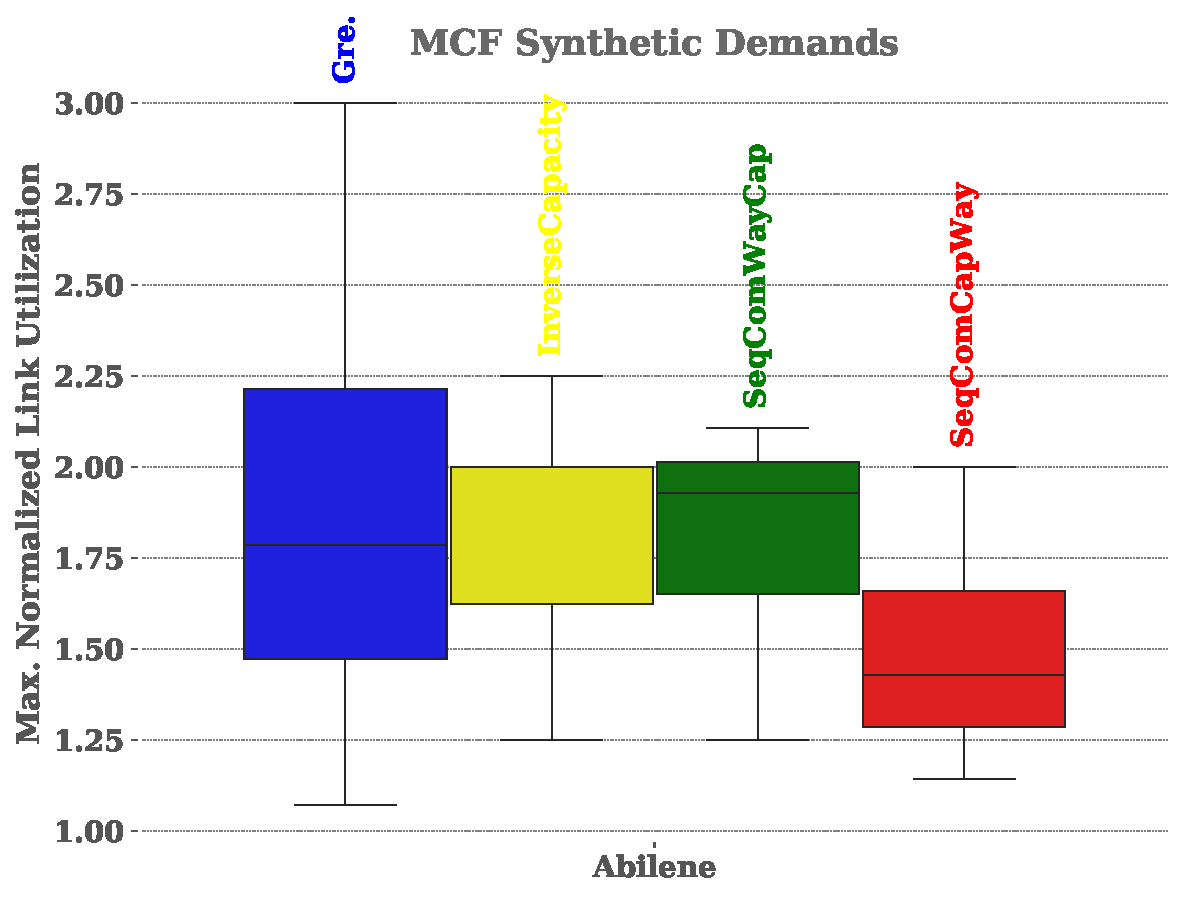
\includegraphics[width=\linewidth]{figures/pouria_all_algorithms_abilene.pdf}
\caption{Vergleich von vier Algorithmen mit syntetischen Anforderungen auf der Abilene-Topologie. Legende: greedy waypoints in blau, inverse capacity in gelb, SeqComWayCap in gr\"un, SeqComCapWay in rot.}
\label{fig:pouriaBoxplotSynthetic}
\end{figure}
% Das [h] kann weg, dann findet Tabelle automatisch den besten Platz
\begin{figure}
\centering
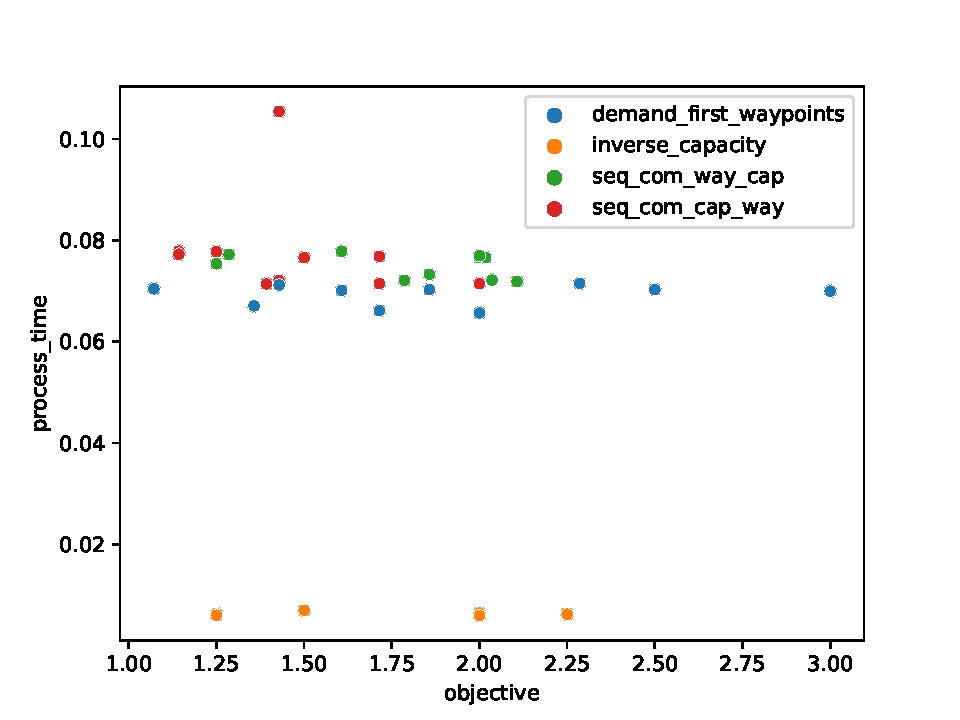
\includegraphics[width=\linewidth]{figures/pouria_colored_scatter_plot_results_all_algorithms.pdf}
\caption{Vergleich von vier Algorithmen mit syntetischen Anforderungen auf der Abilene-Topologie. Legende: greedy waypoints in blau, inverse capacity in gelb, SeqComWayCap in gr\"un, SeqComCapWay in rot.}
\label{fig:pouriaScatterSynthetic}
\end{figure}
% Das [h] kann weg, dann findet Tabelle automatisch den besten Platz
\begin{figure}
\centering
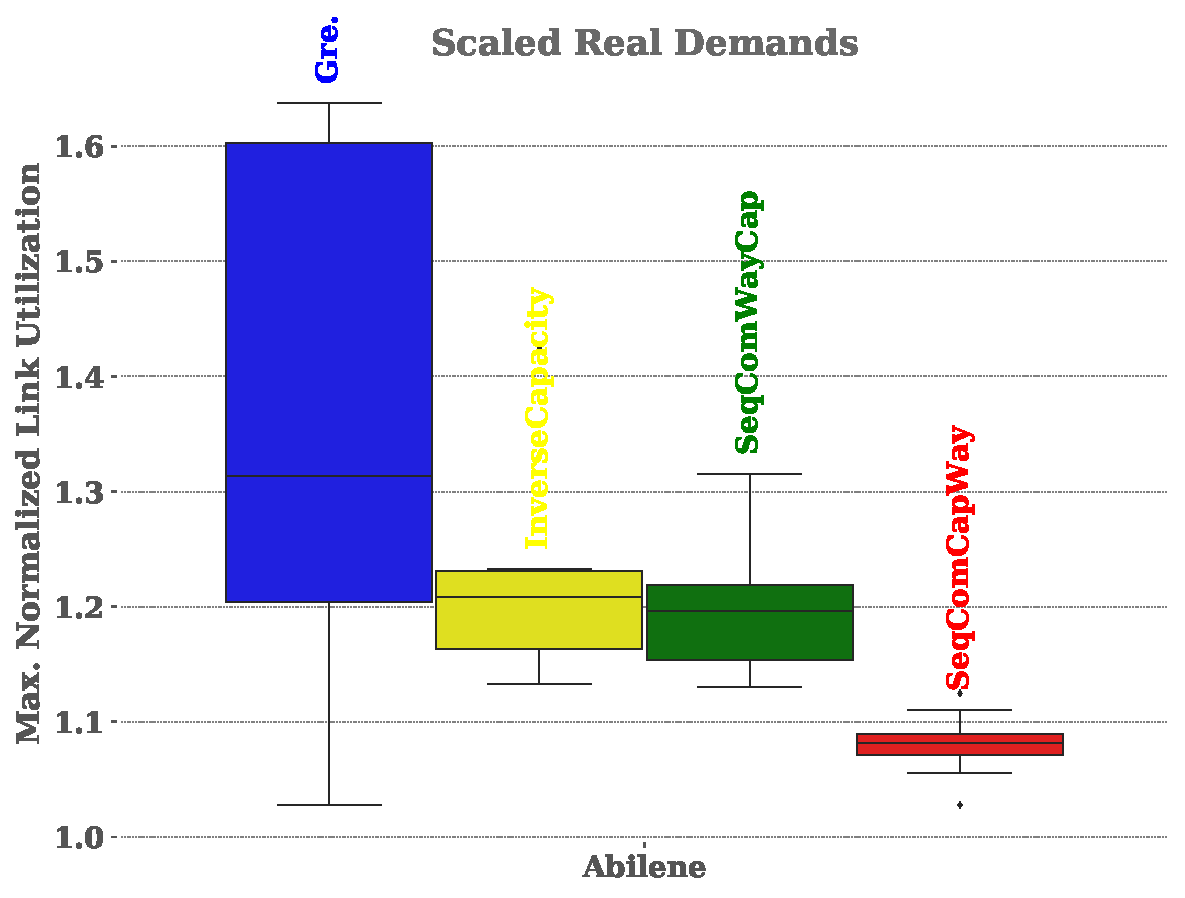
\includegraphics[width=\linewidth]{figures/pouria_real_demands.pdf}
\caption{Vergleich von vier Algorithmen mit realen Anforderungen auf der Abilene-Topologie. Legende: greedy waypoints in blau, inverse capacity in gelb, SeqComWayCap in gr\"un, SeqComCapWay in rot.}
\label{fig:pouriaBoxplotReal}
\end{figure}
% Das [h] kann weg, dann findet Tabelle automatisch den besten Platz
\begin{figure}
\centering
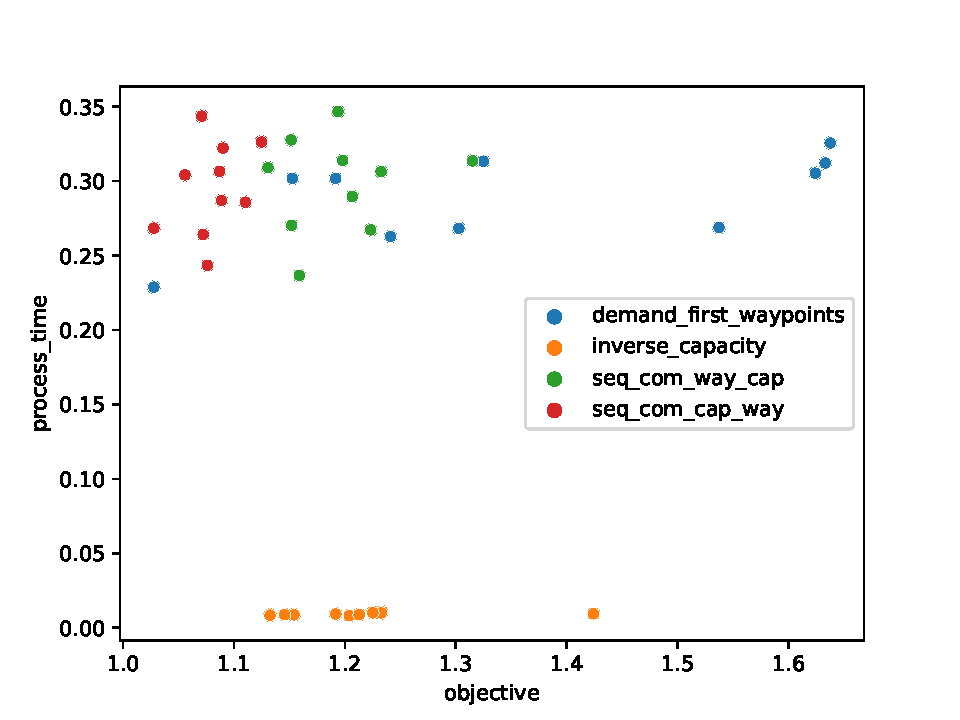
\includegraphics[width=\linewidth]{figures/pouria_colored_scatter_plot_results_real_demands.pdf}
\caption{Vergleich von vier Algorithmen mit syntetischen Anforderungen auf der Abilene-Topologie. Legende: greedy waypoints in blau, inverse capacity in gelb, SeqComWayCap in gr\"un, SeqComCapWay in rot.}
\label{fig:pouriaScatterReal}
\end{figure}
Die Abbildungen \ref{fig:pouriaBoxplotSynthetic} und \ref{fig:pouriaBoxplotReal} geben eine Antwort auf Frage 1.
Sie zeigen, 
dass die sequentielle Kombination beider Algorithmen in beiden F\"allen mindestens genauso gut ist wie eines seiner Bestandteile. 
Im Fall von $SeqComCapWay$ ist dieser im Durchschnitt sogar besser als beide Algorithmen.
Dies l\"asst sich darauf zur\"uckf\"uhren, 
dass die Kantengewichte durch den Algorithmus $inverse\_capacity$ zu Beginn verbessert werden 
und anschlie\ss end durch den zweiten Algorithmus weiter verbessert werden, falls m\"oglich.
Im Folgenden wird daher nur noch auf die sequentielle Kombination \emph{SeqComCapWay} (in rot) eingegangen.\newline
Die Abbildungen \ref{fig:pouriaScatterSynthetic} und \ref{fig:pouriaScatterReal} hingegen sind relevant f\"ur die Frage 2. 
Diese zeigen einen etwas genaueren Blick auf die Rechenergebnisse geplottet \"uber die daf\"ur ben\"otigte Zeit.
Hier kann auch direkt gesehen werden, dass $inverse\_capacity$ mit Abstand der schnellste hier verwendete Algorigthmus ist.
Dies ist besonders vorteilhaft, da es bedeutet, 
dass die sequentielle Kombination aus $inverse\_capacity$ und $greedy\_waypoints$ kaum l\"anger mehr Berechnungszeit ben\"otigt als $greedy\_waypoints$ alleine.
Somit konnte empirisch gezeigt werden, 
dass in diesem "vereinfachten" Beispiel die Kombination der oben genannten Algorithmen nicht nur im Durchschnitt bessere MLU-Ergebnisse liefert, 
sondern das auch in derselben Zeit erledigt.
Und somit l\"asst sich die Frage der Rechtfertigung auslagern.
In allen F\"allen, in denen der $greedy\_waypoints$-Algorithmus gerechtfertigt ist,
ist auch die oben genannte Kombination gerechtfertigt.\newline
Da es aus Zeitgr\"unden sowie mangelnder Rechenressourcen nicht so einfach m\"oglich war,
diese Algorithmen auf sehr gro\ss en Tologien zu testen,
kann nicht mit Sicherheit gesagt, wie hoch die Berechnungszeit in Topologien mit 50 oder mehr Knoten wirklich ist.
Daher ist es schwer, diese Algorithmen (mit Ausnahme von $inverse\_capacity$ in solchen Topologien dynamisch zu verwenden.
\subsubsection{Centrality-Metriken mit inverse capacity}
Hier war der Gedanke, den Algorithmus inverse capacity, der statisch auf der Topologie (also Demand unabhängig) berechnet wird, mit Zentralitätswerten zu erweitern.

Ich habe mich für die Zentralitätswerte closeness-, eigenvector- und betweeness-Zentralität entscheiden.
Im Folgenden werden nun die Zentralitätsmetriken definiert (Definitionen aus \cite{guide}), und dann erläutet warum diese ausgewählt wurden:

\begin{enumerate}
    \item \textbf{Adjazenzmatrix}
    Adjazenzmatrix \texttt{A} wird benutzt um einen Graphen als Matrix darzustellen.

    Für dies gilt: $a_{ik} = \begin{cases} 1 & \text{wenn Knoten i und k eine Kante verbindet}, \\ 0 & \text{sonst} \end{cases}$ 

    \item \textbf{closeness-centrality}
    Wie im Namen bereits benannt, berechnet diese Metrik, wie nah ein Knoten allen anderen ist.
    Die closeness-centrality $c_i$ des Knoten $i$:
    \begin{center}
        $c_i = \frac{1}{\sum_{j\neq i} H(\mathcal{P}_{i\rightarrow j})}$
    \end{center}
    $\mathcal{P}_{i\rightarrow j}$ ist der kürzeste Pfad von Knoten i nach Knoten j.
    
    $H(\mathcal{P}_{i\rightarrow j})$ ist die Anzahl an Kanten, die genutzt werden müssen, um von Knoten $i$ nach Knoten $j$ zu kommen.
    
    Je höher die closeness-Metrik, desto zentraler ist der Knoten im Graph. 
    
    \item \textbf{betweenness-centrality}
    Die betweenness-centrality gibt das Verhältnis aller kürzesten Wege, die durch einen Knoten $i$ führen, zur Menge aller kürzesten Wege an.
    
    Die betweenness-centrality eines Knoten $i$:
    \begin{center}
        $b_i = \sum_{s,t\in \mathcal{N}} \frac{|\mathcal{P}_{s\rightarrow t}(i)|}{|\mathcal{P}_{s\rightarrow t}|}$    
    \end{center}
    wobei $|\mathcal{P}_{s\rightarrow t}|$ die Anzahl aller kürzesten Wege von $s$ nach $t$ ist und $|\mathcal{P}_{s\rightarrow t}(i)|$ die Anzahl dieser Wege, die durch den Knoten $i$ verlaufen. 
    
     
    \item \textbf{eigenvector-centrality):}
     
     Die eigenvektor-centrality $x_i$ eines Knotens $i$ ist das $i$-te Element des Eigenvektors, die dem größten Eigenwert $\lambda_1$ der Adjazenz-Matrix A entspricht.
     
     Die Formel zur Berechnung lautet:
     \begin{center}
     $x_i = \frac{1}{\lambda_1}\sum^N_{k=1}a_{ik}x_k$
     \end{center}
     
     Hat ein Knoten einen hohen eigenvektor-centrality, lässt sich folgern, dass der Knoten mit anderen wichtigen Knoten verbunden ist.

\end{enumerate}

Die closeness-centrality wurde gewählt, da die closeness aussagt wie vielen Kanten ein Knoten von allen anderen entfernt ist, daher potenziell viele Datenstörme durch diesen Knoten fließen können.
Die betweeness-centrality wurde gewählt, da Knoten mit hoher betweeness, an vielen kürzesten Wegen beteiligt sind, hier also das Risiko für Link Überlastung hoch ist.
Die eigenvector-centrality wurde gewählt, da eine hohe eigenvector-centrality darauf schließen lässt, dass der Knoten ein guter "Verteiler"-Knoten im Netz ist.

In der tatsächlichen Implementierung wurden die centrality Berechnungen von NetworkKit benutzt, und dort zusätzlich noch normalisiert.


Um inverse capacity mit den centrality Werten zu verrechnen wird folgende Formel genutzt (für die Kante von i nach j:
\begin{center}
    $new\_weight_{ij} = inverse\_capacity\_weight * \frac{CentralityNode_i + CentralityNode_j}{2}$
\end{center}

In \ref{fig:kai_p1_results} gibt es neben \$centralityInverseCapacity auch noch \$centralityCapacity, dass ist der Algorithmus ohne InverseCapacity, also:

\begin{center}
    $new\_weight_{ij} = weight * \frac{CentralityNode_i + CentralityNode_j}{2}$
\end{center}

Diese dürften schlecht abschneiden, sind hier jedoch mit dabei, um den Unterschied zu unterstreichen.


%%Auswertung Projekt 1
\begin{figure}
    \centering
    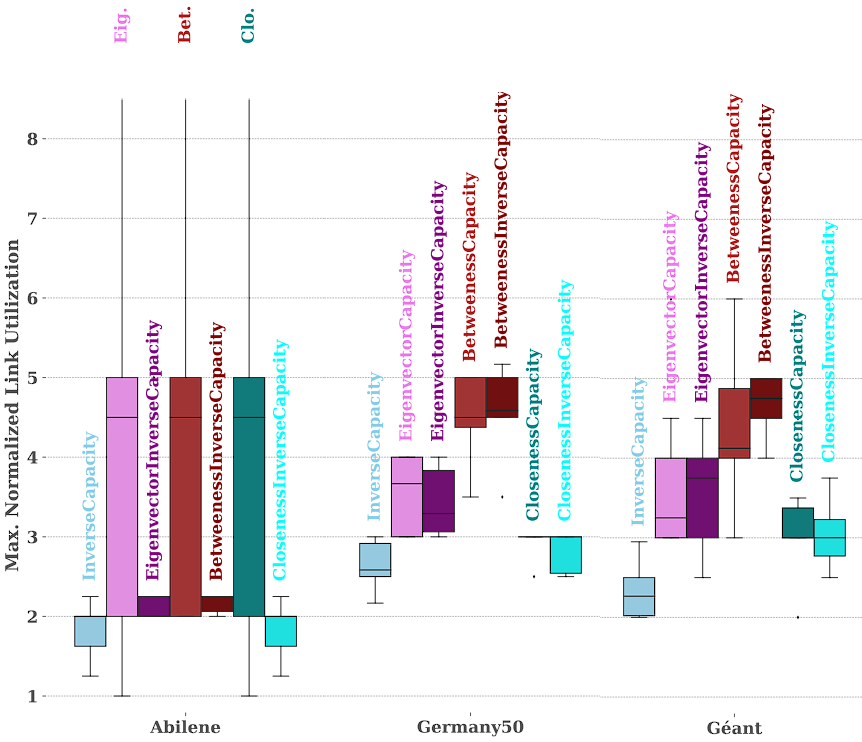
\includegraphics[width=\linewidth]{figures/kai_p1_results.png}
    \caption{Ergebnisse für centrality-inverse-capacity}
    \label{fig:kai_p1_results}
\end{figure}


Wie man in Abbildung \ref{fig:kai_p1_results} zu sehen ist, ist der neue Algorithmus keine Verbesserung auf den getesteten Topologien.
Am schlechtesten schneidet hier der Algorithmus mit der betweeness centrality ab, dicht gefolgt von der eigenvector centrality.
Die closeness centrality schneidet mit am besten ab und ist im Beispiel für "Abilene" gleich auf mit inverse capacity.
Die Algorithmen ohne inverse capacity sind, schlechter, jedoch (abgesehen von Abilene) nah an den anderen Algorithmen dran.

Die schlechtere Performance kann dadurch erklärt werden, dass die weights der Kanten bei reinem Inverse Capacity, zwei kürzeste Wege zwischen zwei Knoten entstehen lassen, und diese durch die centralities dann, durch die neue Gewichtung, nur noch einen kürzesten Weg haben.
Dadurch werden dann einzelne Links überlastet und die MLU wird schlechter.
\subsection{Experimente zu Projekt 2}
In diesem Projekt ging es darum, die eigene algorithmische Idee zu nehmen und in einem virtuellen Netzwerk\footnote{\url{https://github.com/nikolaussuess/nanonet}, siehe Abschnitt \ref{sec:resouces}} zu testen. 
Dieses Projekt wurde ebenfalls mithilfe eines bereits existierenden Repositories\footnote{\url{https://github.com/fruitiestPunch/FaPro_P2}, siehe Abschnitt \ref{sec:resouces}} bearbeitet.
\subsubsection{Sequential combination aus inverse capacity und demand first waypoints}
\label{sec:seq_com_p2}
Zum Testen dieses Algorithmus wurde eine vereinfachte Topologie mit wenigen Anforderungen erstellt.
In Abbildung \ref{fig:pouriaSimpleTopology} ist die finale Topologie zu sehen, 
wobei hier bereits der $inverse\_capacity$-Algorithmus darauf ausgef\"uhrt wurde.
In der Tabelle \ref{tab:pouriaSimpleTopology} sind die beiden Anforderungen sowie deren Start- und Endknoten angegeben.
Die Timeouts in diesen Experimente haben zu einigen Problemen gef\"uhrt.
Da der Rechner auf dem speziell dieser Algorithmus getestet wurde,
relativ schwach war (4GB RAM), wird vermutet, 
dass die Timeouts
\footnote{\url{https://github.com/nikolaussuess/nanonet}, siehe Abschnitt \ref{sec:resouces}}
\footnote{\emph{nanonet\_batch.py} aus \url{https://github.com/fruitiestPunch/FaPro_P2}, siehe Abschnitt \ref{sec:resouces}}
\begin{verbatim}
  at now+2min
\end{verbatim}
und 
\begin{verbatim}
  sleep(8 * 60)
\end{verbatim}
nicht ausgereicht haben, sodass einige der Prozesse fr\"uhzeitig abgerbochen wurden.
Abbildung \ref{fig:pouria_boxplot_no_boxes} zeigt dabei die MLU-Werte aller drei Algorithmen im Vergleich.
Die Tatsache, dass die Boxplots hier nur als Striche dargestellt werden, weist daraufhin, dass es keine Streuung in den finalen Ergebnissen gab,
was auf das fr\"uhzeitige Abbrechen einiger Rechenprozesse zur\"uckgef\"uhrt werden kann.
\begin{figure}
\centering
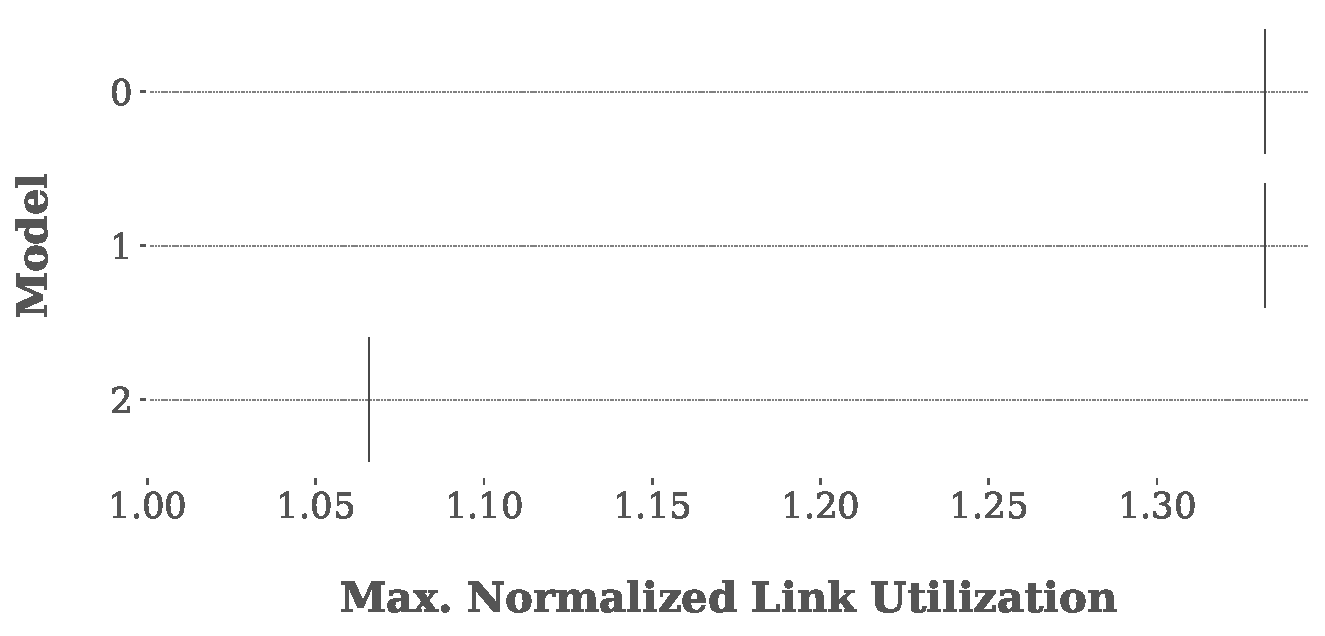
\includegraphics[width=\linewidth]{figures/pouria_boxplot_no_boxes.pdf}
\caption{Vergleich von drei Algorithmen als Boxplotdiagramme. Legende: 0 = Joint, 1 = Weights, 2 = Pouria.}
\label{fig:pouria_boxplot_no_boxes}
\end{figure}
% Das [h] kann weg, dann findet Tabelle automatisch den besten Platz
\begin{figure}
\centering
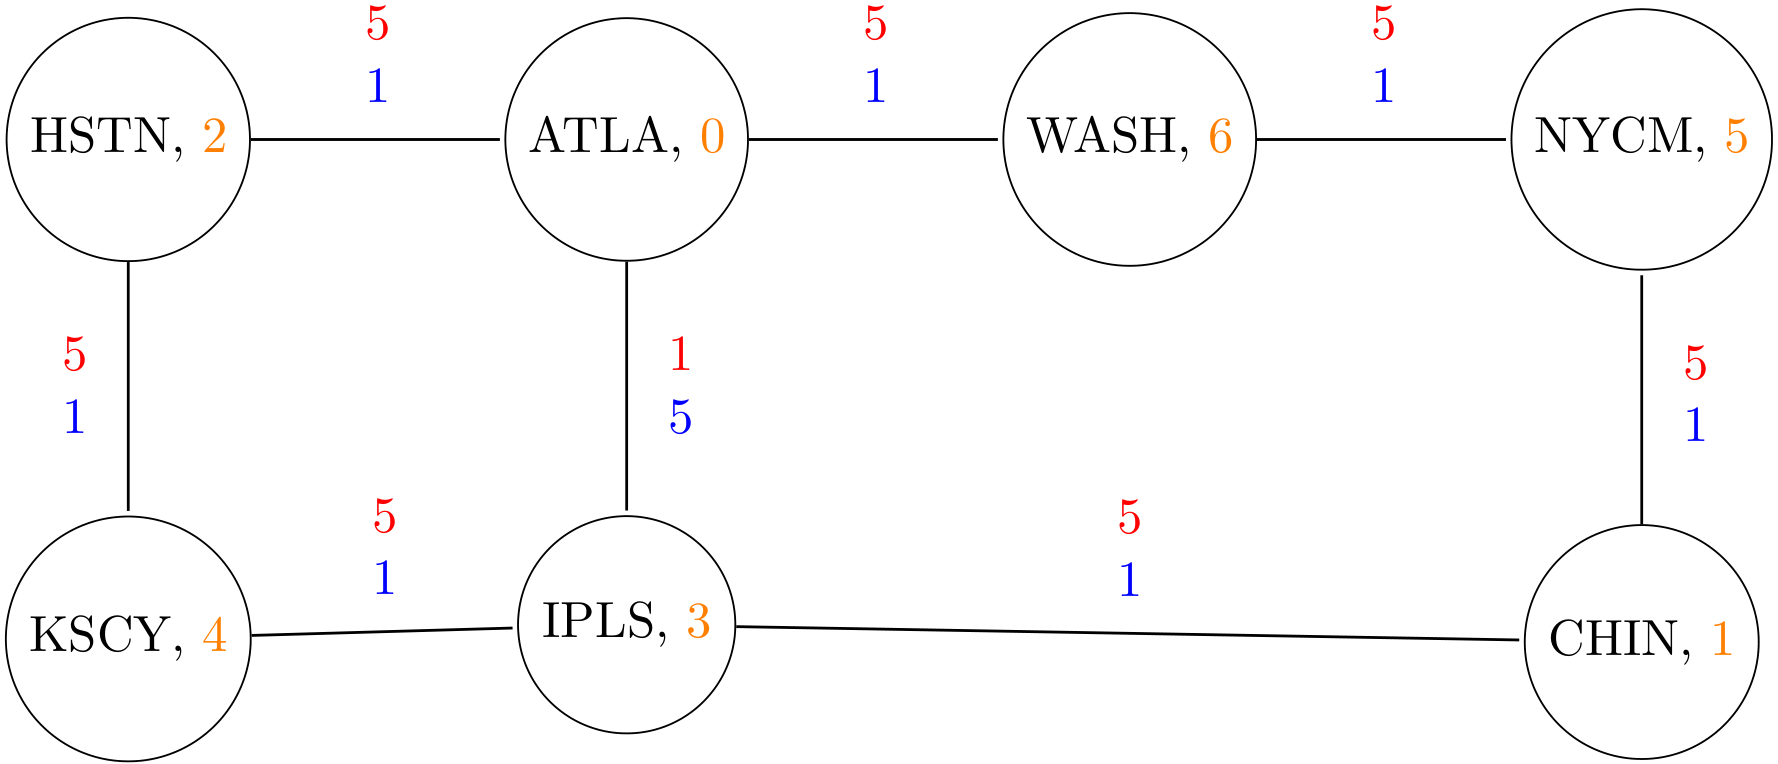
\includegraphics[width=\linewidth]{figures/pouria_simple_topology.png}
\caption{Vereinfachte Netzwerktopologie [Anlehnung an Abilene]. Legende: Kapazit\"aten in rot, Gewichte in blau.}
\label{fig:pouriaSimpleTopology}
\end{figure}
% Das [h] kann weg, dann findet Tabelle automatisch den besten Platz
\begin{table}
\caption{Vereinfachte Anforderungstabelle. Vollst\"andige Tabelle unter \url{https://github.com/fruitiestPunch/FaPro_P2/tree/master/pouria}}
\label{tab:pouriaSimpleTopology}
\begin{tabular}{cccc}
\toprule
$\downarrow$ von, nach $\rightarrow$&IPLS&WASH&$\cdots$\\
\midrule
ATLA & 5 & &\\
IPLS & & 7 & \\
$\vdots$ & & & \\
\bottomrule
\end{tabular}
\end{table}
\subsubsection{Centrality-Metriken mit inverse capacity}

\begin{figure}
    \centering
    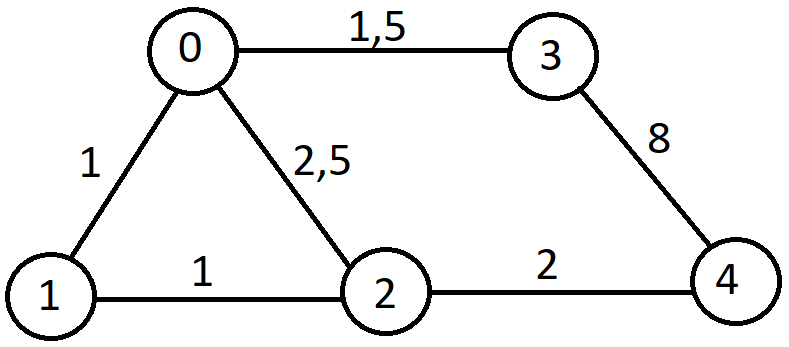
\includegraphics[width=\linewidth]{figures/kai_p2_baseTopo.png}
    \caption{Topologie für die Tests des Algorithmus centrality Metriken mit inverse capacity}
    \label{fig:kai_p2_baseTopo}
\end{figure}
Die Topologie für die Tests der centrality Metriken mit inverse capacity ist die in Abbildung \ref{fig:kai_p2_baseTopo}
Es gibt zwei Demands, einmal von 0 nach 4 mit Größe 1, und einmal von 3 nach 4 mit Größe 8.
Außerdem wurde hier nur die centrality Metrik closeness benutzt, da diese im ersten Projekt am besten der drei Metriken abgeschlossen hat.

Warum diese Topologie genutzt wurde, wird klar wenn man sich die Ergebnisse anschaut.
Wie man in Abbildung \ref{fig:kai_p2_results} sehen kann, performt auf dieser Topologie der Algorithmus besser als inverse capacity.
Der Grund dafür wird in Abbildung \ref{fig:kai_p2_AdTopo} verdeutlicht.
Inverse capacity schickt beide Demands über die Kante zwischen 3 und 4, dadurch wird diese überlastet.
Inverse capacity mit der closeness Metrik schick ein Demand von 3 nach 4 und den anderen über 0 nach 2 nach 4 und verhindert dadurch die Überlastung.

\begin{figure}
    \centering
    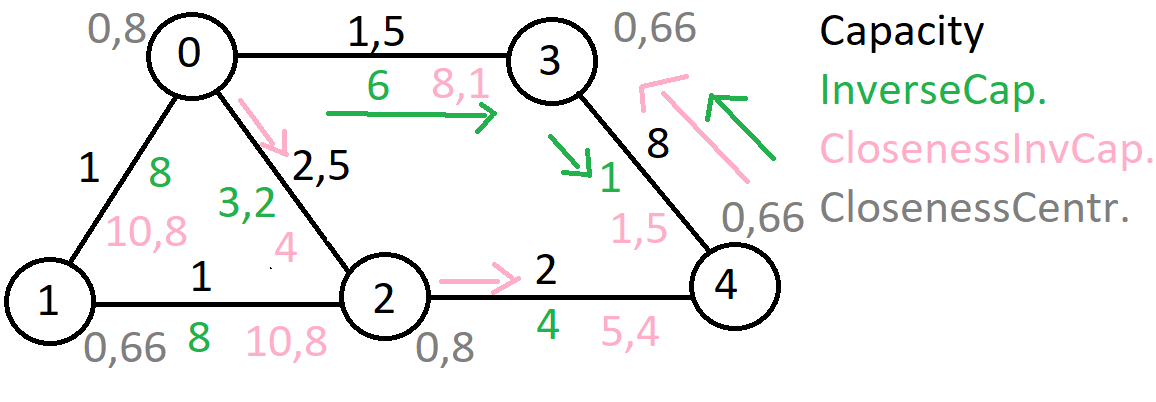
\includegraphics[width=\linewidth]{figures/kai_p2_TopoAd.png}
    \caption{Topologie mit ausgerechneten Werte, Pfeile geben die jeweils genommenen Pfade an}
    \label{fig:kai_p2_AdTopo}
\end{figure}

\begin{figure}
    \centering
    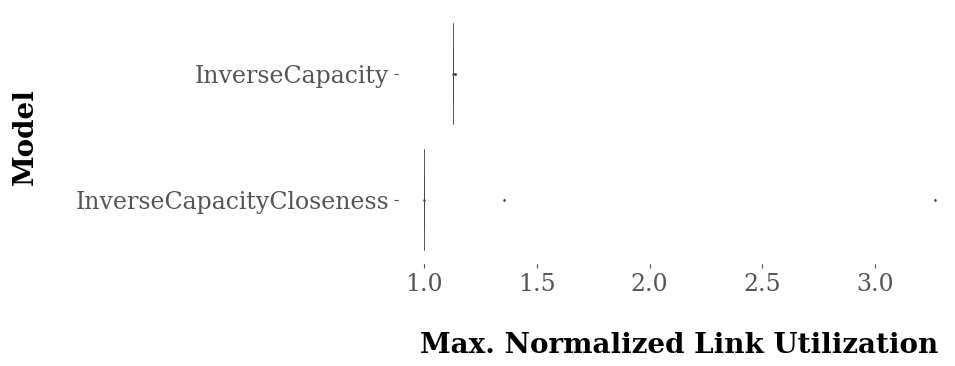
\includegraphics[width=\linewidth]{figures/kai_p2_results.png}
    \caption{Ergebnisse für Algorithmus centrality Metriken mit inverse capacity}
    \label{fig:kai_p2_results}
\end{figure}


\section{Replikation}
Im Folgenden werden die Ergebnisse und Einsichten der Replikationen von Gruppe 2 vorgestellt.
\subsection{Replikation zu Projekt 1}
Die Replikation von diesem Projekt war zu Beginn leider etwas schwierig, weil in beiden F\"allen Abh\"angigkeiten fehlten.
Ein gro\ss es Problem beim Replizieren des Deep-Learning-Projekts war, dass sich der Prozess nach einer Weile selbstst\"andig beendet hat.
Die Vermutung liegt nahe, dass der Rechenaufwand so hoch war, dass der Rechner ab einem bestimmten Zeitpunkt den Prozess selbst beendet hat.
Ein weiteres Problem beim Replizieren waren die Fehlermeldungen und Abbr\"uche beim Plotten. 
\begin{figure}
\centering
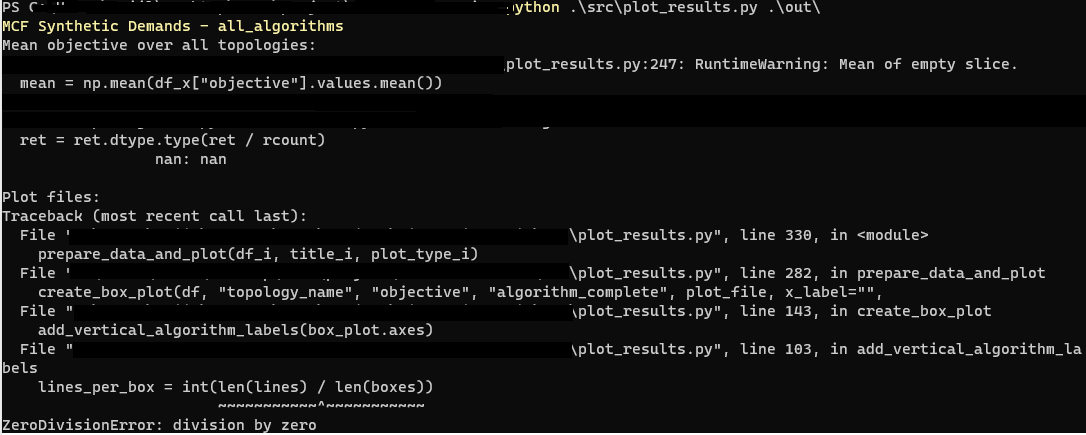
\includegraphics[width=\linewidth]{figures/repl_p1_plottererror.png}
\caption{Plotting-Fehlermeldung im Terminal}
\label{fig:repl_p1_plottererrror}
\end{figure}
Diesem und \"ahnlichen Fehlern sind wir bei unser Bearbeitung ebenfalls begegnet und die Behebung hat sich als au\ss erordentlich schwierig erwiesen, weil dieser "Plottererror" innerhalb einer Python-Bibliothek liegt.
Abbildung \ref{fig:repl_p1_plottererrror} zeigt einen solchen Fehler,
welcher sich hartn\"ackig auch nach einigen Anpassungsversuchen weiterhin erhalten hat.
\subsection{Replikation zu Projekt 2}
Die Replikation des Codes aus Gruppe 2 lief im Allgemeinen problemlos, wie die Abbildungen \ref{fig:repl_p2_daniel2} und \ref{fig:repl_p2_zixiang_10} zeigen.
\begin{figure}
\centering
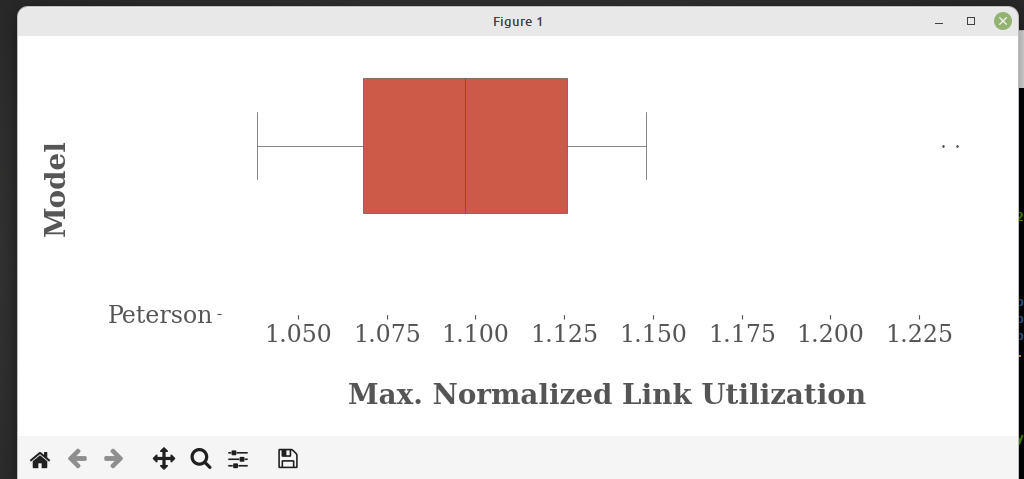
\includegraphics[width=\linewidth]{figures/repl_p2_daniel2.png}
\caption{Ergebnisdiagramm des Codes von Gruppe 2}
\label{fig:repl_p2_daniel2}
\end{figure}
\begin{figure}
\centering
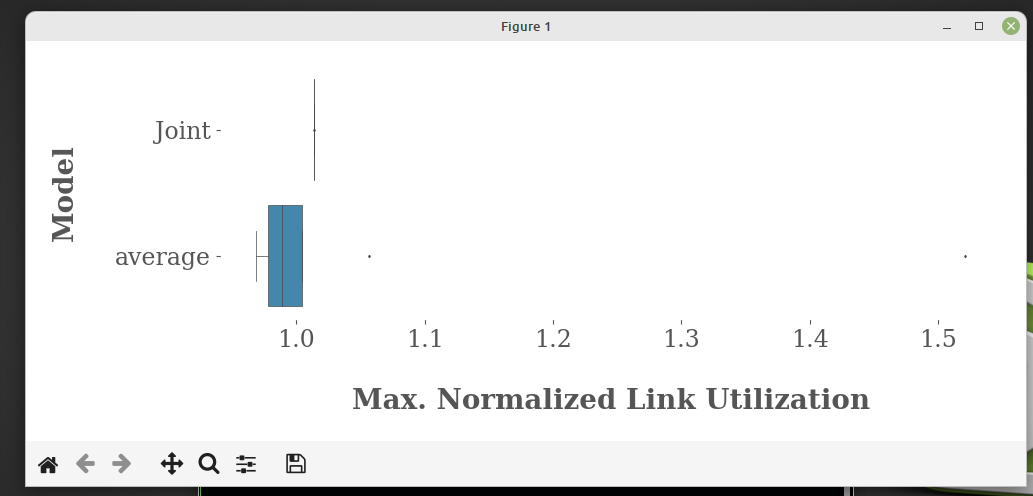
\includegraphics[width=\linewidth]{figures/repl_p2_zixiang_10.png}
\caption{Ergebnisdiagramm des Codes von Gruppe 2}
\label{fig:repl_p2_zixiang_10}
\end{figure}
Ein Problem, welches auch innerhalb unserer Gruppe aufgetaucht ist,
waren die identischen Werte nach Beendigung der \emph{nanonet\_batch.py}-Datei.
Wie bereits in Abschnitt \ref{sec:seq_com_p2} erw\"ahnt, liegt dieses Problem vermutlich an mangelnder Rechenleistung w\"ahrend des Berechnungsprozesses.
Nach wiederholtem Ausf\"uhren des Codes konnte dieses Problem jedoch behoben werden.
\begin{figure}
\centering
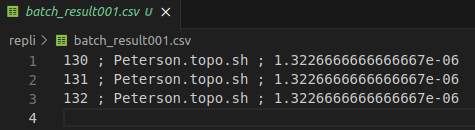
\includegraphics[width=\linewidth]{figures/repl_p2_daniel1.png}
\caption{Ergebnis-CSV-Datei mit identischen MLU-Werten in jeder Zeile}
\label{fig:repl_p2_daniel1}
\end{figure}
\section{Zusammenfassung}
Es kann gesagt werden, dass wir w\"ahrend des Fachprojekts vieles lernen konnten, 
insbesondere Dinge, die nicht notwendigerweise im Stundenplan stehen, 
aber gerade auf der akademischen Laufbahn als Standard angesehen werden.
Das Nachstellen einer wissenschaftlichen Arbeit hat sich als nicht-trivial erwiesen 
und das obwohl diese Arbeit f\"ur ihre hohe Reproduzierbarkeit ausgezeichnet wurde.
Dies l\"asst leider nur auf eine Folgerung schlie\ss en; viele andere wissenschaftlichen Arbeiten lassen sich viel schwerer oder gar nicht nachstellen. 
W\"ahrend des Replizierens der Projekte der anderen Gruppen war es ebenfall \"uberraschend, 
das selbst wenn unsere Gruppen alle an denselbem Hauptprojekt gearbeitet haben 
und theoretisch alle dieselben Pakete verwendeten, 
es manchmal dennoch zu Replikationsschwierigkeiten kam.
Allerdings war es auch eine sch\"one Erfahrung in einer Gruppe an so einem Projekt zu sitzen 
und die Probleme intern sowie mit den anderen Gruppen besprechen zu k\"onnen.
Das hat nicht nur zu einem gr\"o\ss eren Zusammengeh\"origkeitsgef\"uhl gef\"uhrt,
sondern wir haben auch gelernt, kollaborativ gemeinsame Schwierigkeiten zu l\"osen. 
\section{Ausblick}
Aufgrund der relativ kurzen Bearbeitungszeit und den begrenzten Rechenkapazit\"aten unserer eigenen Computer war es etwas schwer, unsere Algorithmen, insbesondere in Projekt 2, auf gro\ss en Topologien zu testen.
Dies kann dazu f\"uhren, dass bestimmt Effekte wie Datenstaus, welche gerade in gro\ss en Topologien auftauchen, in kleinen kaum oder gar nicht vorkommen.

\begin{acks}
Vielen Dank an Marvin f\"ur seine Hilfe und Geduld mit unseren Problemen. Ohne seine Hilfe w\"are das alles in der kurzen Zeit sehr viel schwieriger gewesen.
\end{acks}

\bibliographystyle{ACM-Reference-Format}
\bibliography{fapro_bib}

\appendix
\section{Onlineressourcen}
\label{sec:resouces}
Im Rahmen dieses Fachprojekts wurden drei \"offentliche Repositories als Hauptquellen verwendet. Die ersten beiden Repositories \url{https://github.com/fruitiestPunch/FaPro_P1} und \url{https://github.com/fruitiestPunch/FaPro_P2}, welche \emph{forks} von \url{https://github.com/tfenz/TE_SR_WAN_simulation} und \url{https://github.com/nikolaussuess/TE_SR_experiments_2021} sind. Die dritte Hauptquelle stellt \url{https://github.com/nikolaussuess/nanonet} dar, welche zur Erstellung von vom Projekt les- und interpretierbaren Netzwerktopologiedaten verwendet wurde.
\end{document}